\documentclass[12pt]{memoir}
\usepackage{common}

\addbibresource{references}

\title{}
\author{Andrew Head}

\begin{document}

\definition{Title}{Supporting Systematic Code Inspection During Opportunistic Programming}

\definition{Author}{Andrew Head, PhD Student, UC Berkeley}

The purpose of this work is to develop more context-relevant, summative, and rapid-access forms of programming documentation that fit directly into fast-paced opportunistic development practices.
The ultimate goal of this work to enable rapid development of reliable software for end user programmers.
This relates to \texbf{broader impacts}, in particular my shared goal with NSF to \textbf{increased public engagement with science and technology}.

\section{Background}

Clarke~\cite{clarke_what_2007} introduced the persona of an \emph{opportunistic developer} to describe a software developer who writes code in an ``exploratory fashion'' and develops a ``sufficient understanding of a technology to understand how it can solve a business problem''.
Recent studies have confirmed both the prevalence of these coding habits, its benefits, and what I will focus on here, its risks.
Those programming opportunistically likely to incorporate functionality by copying and pasting code, often from online sources~\cite{brandt_two_2009}.
They are more likely to implement functionality from scratch for well-known libraries, instead of reusing existing systems and libraries~\cite{brandt_opportunistic_2008}.
They also practice ``code satisficing'', implementing functionality in a sub-optimal way in order to maintain flow and move on to other functionality~\cite{brandt_opportunistic_2008}.

With the increased pace of development, programmers' focus shifts to code examples rather than the prose that helps programmers understand it~\cite{brandt_two_2009}.
Though this lack of vested attention in documentation is no surprise to any of us.
This is a problem that has been studied well when Carroll proposed minimal instruction~\cite{carroll_nurnberg_1990}.
It is also encapsulated by Alan Blackwell's Attention Investment, which describes how end user programmers (those programming for personal purposes) carefully way the costs of engineering activity against the speed of their perceived benefits~\cite{blackwell_pscyhological_2006}.
Good software engineering principles often lose in this assessment.

The growing comprehensiveness of online documentation~\cite{parnin_crowd_2012} and recent understanding of opportunistic programming provides new opportunities to both build adaptive documentation that is in-situ for web-based programming information seeking, and that builds on this documentation as a source.

Anecdotally, this is a trend I have seen increasingly in the classroom.
If programmers unfamiliar with code cannot be compelled to work with documentation, they will miss out on critical learning opportunities to familiarize themselves with the code that they will inevitably need to debug.
Thorough code understanding is a skill programmers must learn before becoming professionals.

\section{Proposed Research}

I hypothesize that context-relevant, summative programming documentation for opportunistic development can help in the following two ways:
\begin{itemize}[noitemsep]
\item it will lesson the effort to develop solutions to problems that involve unfamiliar software or hardware components
\item it will improve programmers' understanding of unfamiliar libraries
\end{itemize}

I propose three systems to embody the ideas context-relevant, summative documentation.  It is my intent to use these systems to demonstrate the technical work needed to produce context-relevant documentation, and it's potential benefits to the opportunistic developer.  One of these systems has been built and results presented at VL/HCC 2015, a conference on end user programming.  A prototype for the other two have been built, and must undergo further development and evaluation.

\subsection{Tutorons}
Context-relevant descriptions of online code.
Programmers may encounter syntax that they don't understand in web tutorials, as an author assumes the audience's prerequisite knowledge.
A Tutoron is a server-side routine that can detect code examples from arbitrary HTML for tutorial pages, parse them, and automatically synthesize English prose, diagrams, and usage examples.
By navigating in a web browser connected to Tutorons with plugins we provide, programmers can view context-relevant explanations of high-level intent of code and its low level syntax.
An initial in-lab usability study has shown that such adaptive explanations can reduce accesses to external documentation on the Web (Fisher's exact test, $n$ = 9, $p<.01$).

\subsection{StackSkim}
Visual search interface for exploring and selecting code from large collections of similar code examples.
It is often the case that there are many tutorials or code examples that can satisfy a programmer's information need.
StackSkim provides a visual interface to StackOverflow, a popular programming Q\&A site with more than 10,000,000 questions, that enables programmers to skim the most popular classes and programming structures used in collections of dozens of related answers to their questions.
While a preliminary usability study revealed positive qualitative feedback, we have not yet applied this to two challenges I believe to be critical for opportunistic developers: (1) highlighting design differences between snippets such as varying approaches and the rationale in the accompanying text. (2) enabling interleaved inspection of instructional examples to real code, the latter which may reveal more realistic exception handling.
The primary technical contribution for both of these steps will revolve around comparison of pre-parsed code examples from the relatively clean repositories of example and production code on StackOverflow and Github, respectively.

\subsection{CodeConverter}
When developing opportunistically, programmers have a set of go-to tools they rely on to get work done (Brandt et al. 2008).
While langauges may share similar concepts, some have key libraries for performing certain tasks that others don't.
This project proposes an experimental simultaneous method of opportunistic programming langauge learning and application.
With CodeConverter, programmers will be able to program simple statements of one language and see them converted to a new language with accompanying description describing how the code's use varies from typical the source language and how it must be modified.
The evaluation will focus on having programmers from a local hackerspace develop code for an embedded platform with an unfamiliar language but with familiar tasks.
While past work has shown machine translation of programming languages (e.g., something), our contribution will not be in this space, but rather in establishing that for a simple subset of common patterns, programming can be enabled for new platforms on familiar tasks, with improved conceptual knowledge through automatically-generated inline comments instead of external documentation.

\begin{figure}%
  \centering
  \parbox{.45\textwidth}{%
    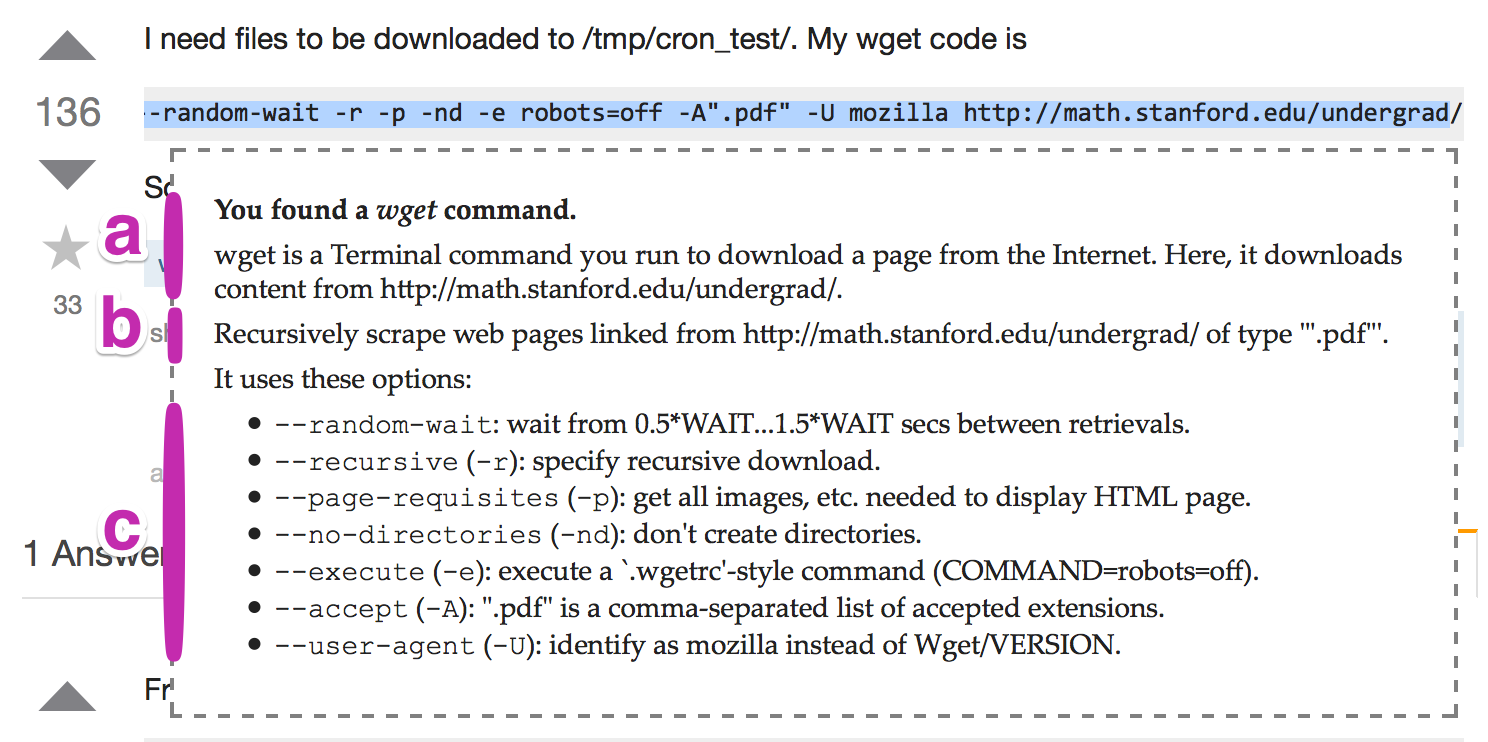
\includegraphics[width=\linewidth]{figures/tutorons_microexplanation}
    \caption{%
      A micro-explanation for a command line generated by a Tutoron with multiple levels of detail 
      (definition, high-level intent, arguments)
    }\label{fig:tutorons_microexplanation}
  }%
  \qquad
  \parbox{.45\textwidth}{%
    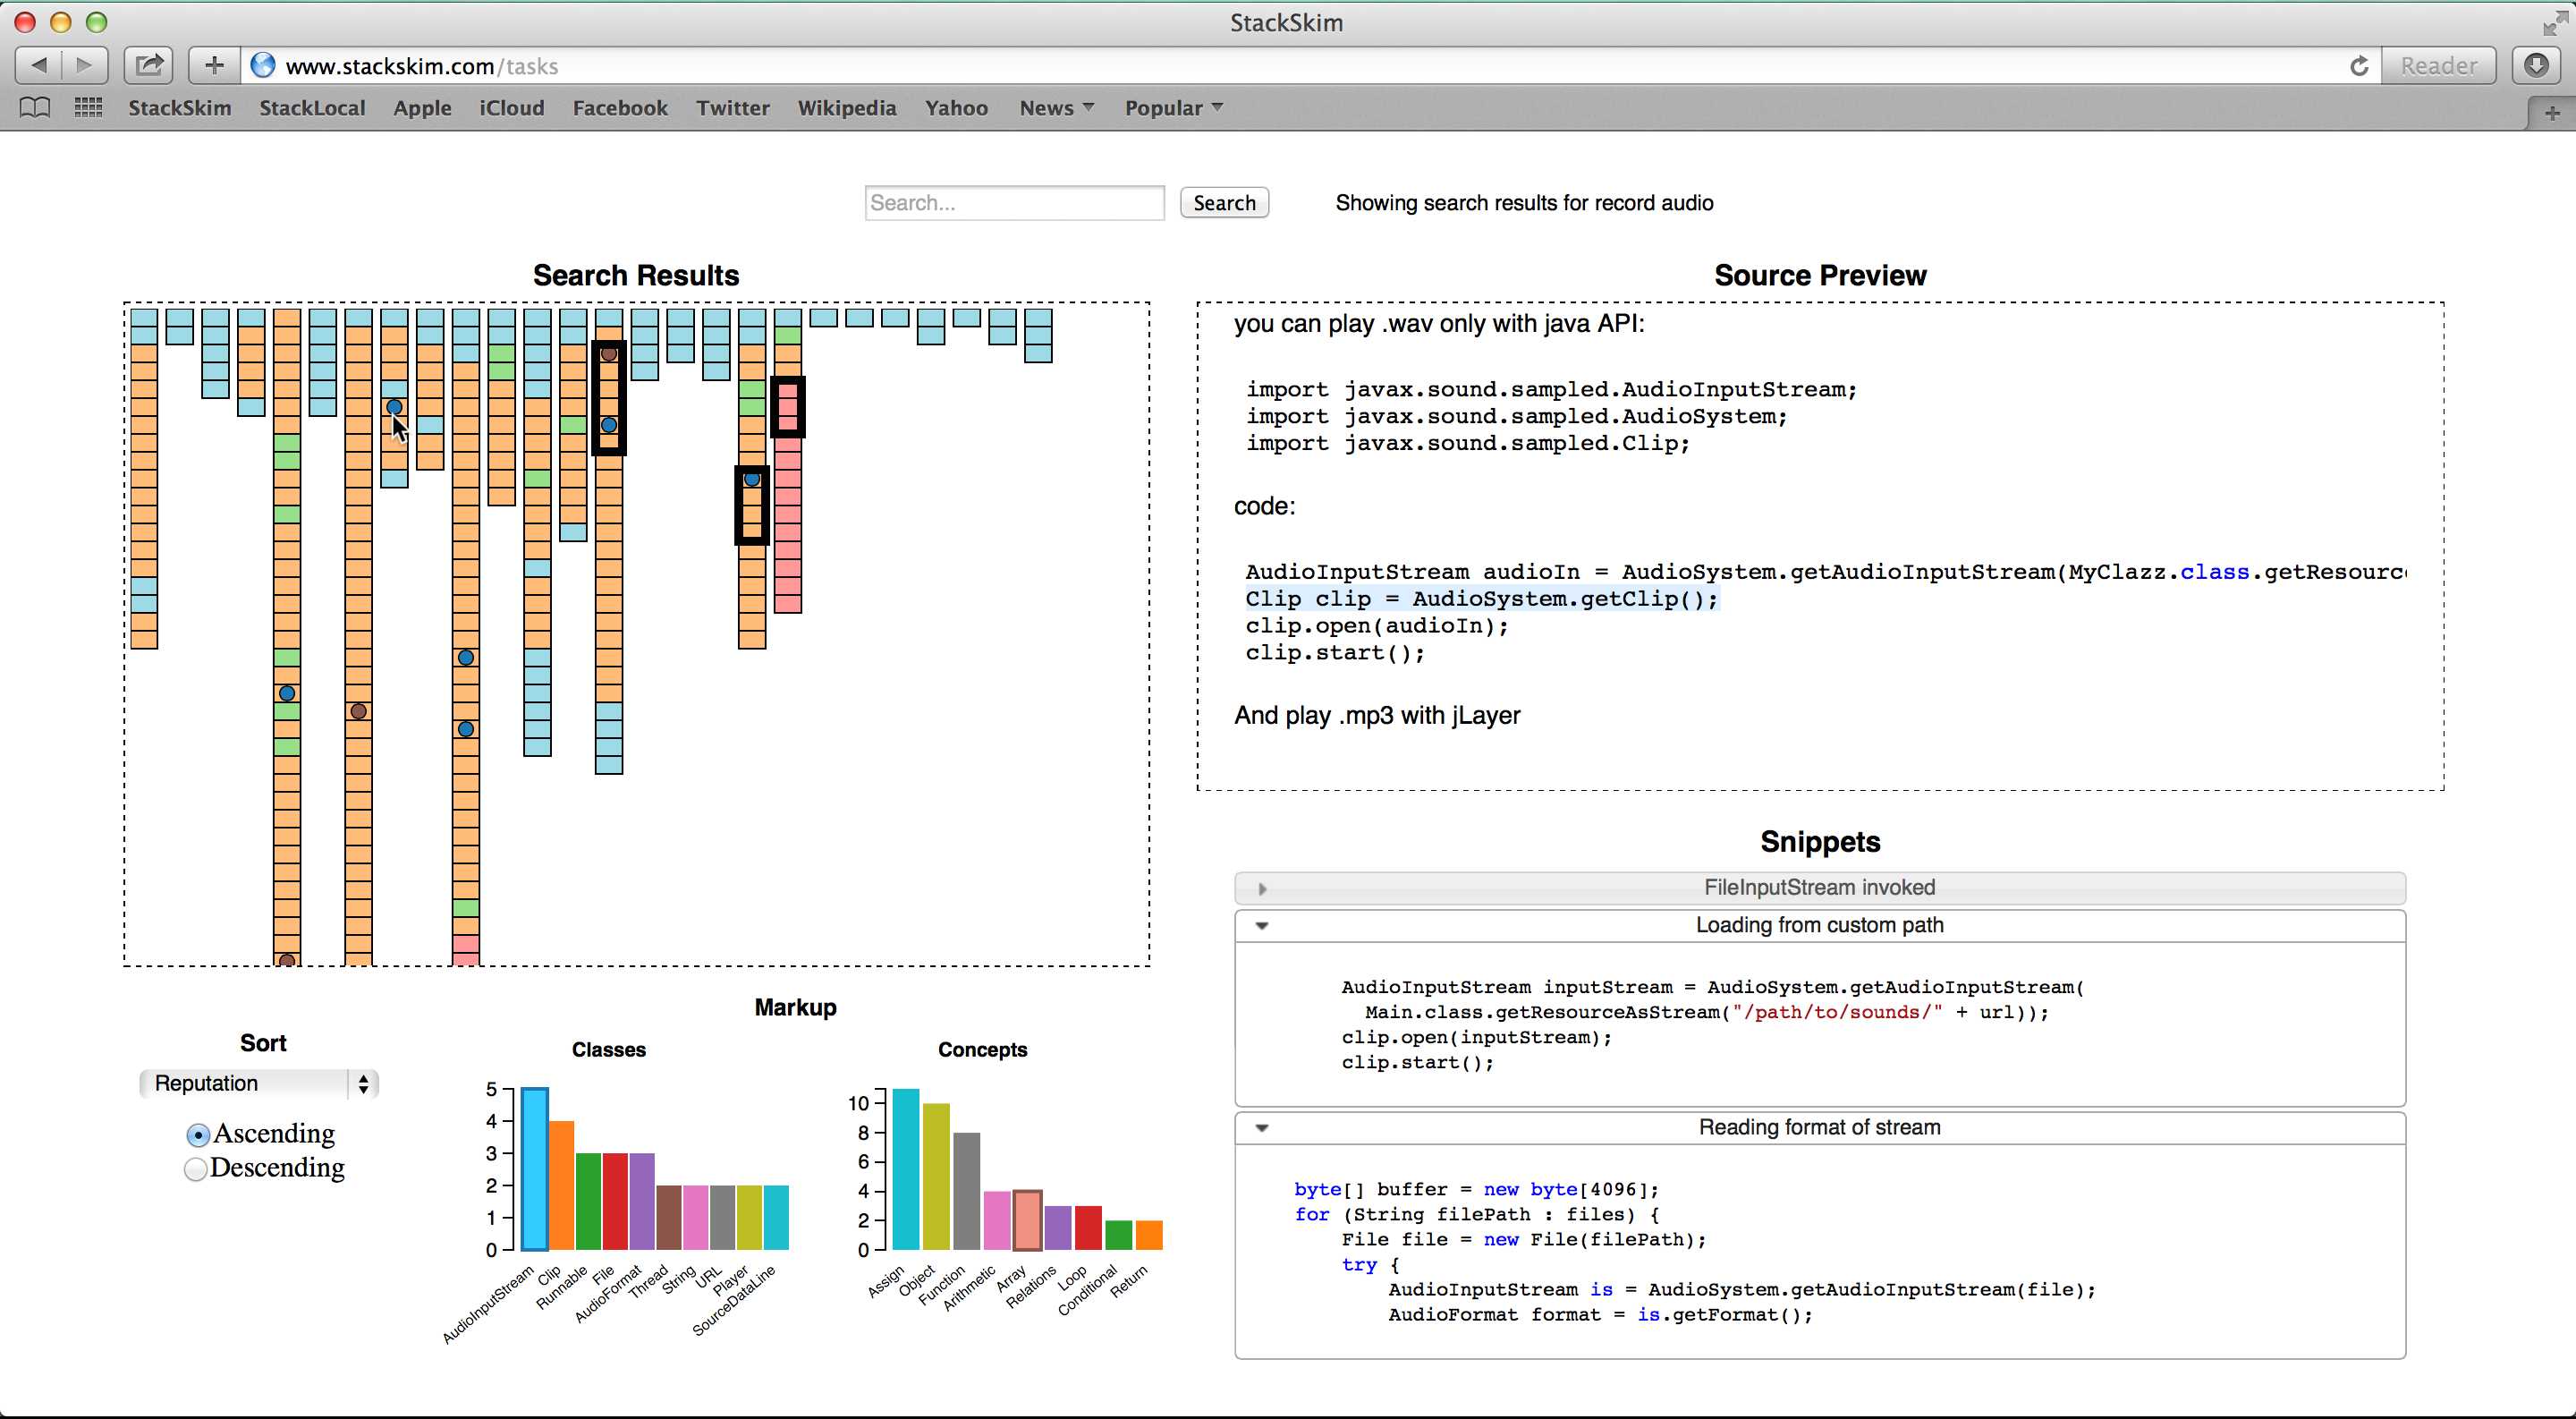
\includegraphics[width=\linewidth]{figures/stackskim_ui}
    \caption{%
      StackSkim, a visual interface for comparing and noticing trends in large collections of code examples that solve the same problem.
    }\label{fig:stackskim_ui}
  }
\end{figure}

\if 0
Point out the number of non-professional programmers.
Also point out crises in developing technologies that are caused by programmers who followed non-systematic practices

This work can be seen as an effort to reconcile the best practices of the ``systematic developer'' with recent tendencies of ``opportunistic'' programming habits.
\textbf{I could add in a mention of Blackwell's Attention Investment model here to mention why it is that programmers may program opportunistically, and why we should and how we can vary incentives and costs.}
Clarke~\cite{clarke_what_2007} introduced the persona of an \emph{opportunistic developer} to describe a software developer who writes code in an ``exploratory fashion'' and develops a ``sufficient understanding of a technology to understand how it can solve a business problem''.
(This contrasts with the \emph{systematic developer}, who writes code defensively and ``develops a deep understanding of a technology before using it''~\cite{clarke_what_2007}.)
In their study of exhibit designers at San Francisco's Exploratorium interactive science museum, Brandt et al.\ reported on a group who engaged in \emph{opportunistic programming} who weren't professional developers~\cite{brandt_opportunistic_2008} but were very much what might be considered as end-user programmers --- those developing code for personal rather than public use~\cite{ko_state_2011}.

Brandt et al.\ associated several habits with opportunistic programming that are counter to what we would hope for students working with code or end-users developing a better understanding of code.
Those programming opportunistically likely to incorporate functionality by copying and pasting code, often from online sources~\cite{brandt_two_2009}.
They are more likely to implement functionality from scratch for well-known libraries, instead of reusing existing systems and libraries~\cite{brandt_opportunistic_2008}.
They also practice ``code satisficing'', implementing functionality in a sub-optimal way in order to maintain flow and move on to other functionality~\cite{brandt_opportunistic_2008}.

While opportunistic programming is powerful in that it allows one to rapidly prototype and ideate and that it reduces the cycle time of editing and debugging code~\cite{brandt_opportunistic_2008}, this behavior discourages the formation of new mental models and an introduction to new tools that should be encouraged for both novice programmers and many end-user programmers.
The author of this proposal observed much of what would be called ``opportunistic'' habits while instructing a user interface design course.
After providing reference code to students for programming interfaces on Android phones and smartwatches, he helped students debug problems related to API reuse and the side effects of mixed code from multiple examples after hearing students self-report to having ``copied and pasted'' code from online tutorials and the slides he distributed.
In light of a prevalence of the ease of opportunistic habits and programmers' ability to copy-and-paste code from an increasingly comprehensive body of crowd documentation online~\cite{parnin_crowd_2012}, I define the goals of my research:

\emph{In my research, I develop and study software artifacts to support systematic inspection of found code from information interfaces programmers use when developing opportunistically.}

The theoretical deliverables of this work is establishing how systematic habits amidst opportunistic practice will improve:
(\emph{a}) programmers' mental models of reused code, libraries and tools used they develop
(\emph{b}) enable more accurate feasibility assessments of upcoming tasks (for example, see~\cite{ko_role_2011})
(\emph{c}) reduce design barriers~\cite{ko_six_2004} when planning new functionality

The artifacts that I develop belong to two themes:
\begin{itemize}[noitemsep]
\item Techniques for automatically generating instructive explanations and demonstrations of found code
\item Interfaces for critical inspection of alternatives when selecting code for reuse
\end{itemize}

I have developed the artifacts that enable exploration within both of these themes, and have published a first paper on the one of the two themes.
Toward the first, a paper I presented at VL/HCC explored techniques for automatically augmenting code in online examples with natural languages explanations and demonstrations of code.\footnote{%
The Tutorons system was implemented as both a browser plugin and a standalone JavaScript library, and can be viewed in action on \url{www.tutorons.com}.
}
We put forward a set of four guidelines to inspire the development of context-sensitive help:
(\emph{a}) leverage multiple representations to illuminate high-level intent and enable low-level understanding of syntax
(\emph{b}) be concise --- skip static explanations and focus on dynamically generated content
(\emph{c}) reappropriate existing documentation
(\emph{d}) inspect code examples on a large scale to support explanations of common usage.
In a nine-participant user study, the system was shown to reduce the number of accesses to external documentation needed to modify online code to perform new tasks.
\textbf{Next steps will include \ldots}
\textbf{Mention the theories used: MLT, layered documentation, Attention Investment}

Towards the second goal, I and co-developer have built a visual search interface for StackOverflow, a popular online programming Q\&A.
In response to Brandt et al.'s recommendations to develop tools that support ``comparing, reasoning about, integrating, and modifying found code''~\cite{brandt_opportunistic_2008}, we developed StackSkim, \emph{a visual search interface for exploring answers to StackOverflow questions that have a multitude of answers}.
The interface offers rapid visual inspection of frequent libraries used for addressing the searcher's programming problem;
through direct manipulation, users can also rapidly collect and compare similar code snippets.
\textbf{Next steps will include \ldots}

Each of these efforts relies on the cultivation of new software artifacts to aid programmers in understanding code during an opportunistic programming task.
Each has already followed and will continue to follow a mixed methods approach of observation and controlled experiments to determine how these tools indeed alter not only the task of opportunistic programming, but also programmers' behavior in selecting, understanding, and using code found online.
We are currently developing a version of Tutorons explanations that we hope will be incorporated into an introductory CS classroom's online textbook to better understand the role of automatic explanations of code for novice programmers.
\textbf{Add some note here about how we intend to run some workshop on clean code reuse habits.}
\fi

\section{References}
\printbibliography[heading=none]

\end{document}
